\documentclass[../../main.tex]{subfiles}

\begin{document}
    
    Simplicial sets can be seen as a generalization of directed multigraphs. Calling the vertices in a multigraph 0-simplices and the edges 1-simplices, each 1-simplex $k_1$ is assigned two 0-simplices $d_0k_1$ and $d_1k_1$, the head and tail vertex of $k_1$ respectively. The maps $d_i$ are called the \emph{face maps} for 1 simplices. This raises the question what exactly an $n$-simplex should be. An $n$-simplex from geometry has $n+1$ vertices and faces, which can all be considered simplices too.

    \begin{example}[2-simplex]
        A $2$-simplex is a triangle, which has three faces(sides) and three vertices, that we will assume are ordered. The order is arbitrary. Each face can be uniquely identified with the vertex opposite of it, which induces an order on the faces too. Having a set of triangles with vertices denoted by $\{0,..,2\}$ we therefore have a face map $d_i$ sending every 2-simplex to its $i$'th edge which is a $0$-simplex. This can in turn be sent to its $2$ faces which are vertices of a triangle. 
        
        Therefore the situation could modeled as follows. There are three sets $X_2$, $X_1$ and $X_0$ of $2$-, $1$- and $0$-simplices with maps $d_i: X_n \to X_{n-1}, i \in \{0,.., n\}$ between them. The structure is realized by observing that $d_0d_1 = d_0d_0$, $d_1d_2 = d_1d_1$ and $d_0d_2 = d_1d_0$ must hold as the vertex at the head of an edge must be at the tail of the following. In other words, these relations arise from the fact that any vertex can be reached in two ways because it is part of two sides.

        \begin{figure}[H]
            \begin{subfigure}[b]{0.3\textwidth}
                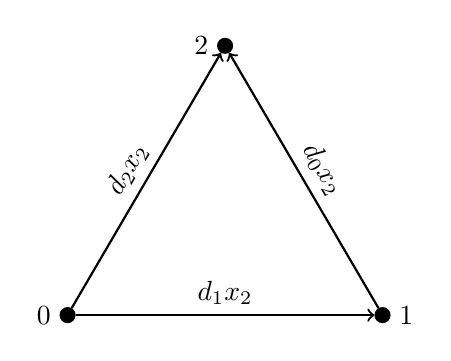
\begin{tikzpicture}[thick, scale=2]
                    \node[circle, draw=black, fill=black, inner sep=0pt, minimum size=5pt,name=0] at (0,0) {};
                    \node[xshift=-2mm] at (0.west) {0};
                    
                    \node[circle, draw=black, fill=black,inner sep=0pt, minimum size=5pt, name=1] at (1,1.71) {};
                    \node[xshift=-2mm] at (1.west) {2};
                    
                    \node[circle, draw=black, fill=black,inner sep=0pt, minimum size=5pt, name=2] at (2,0) {};
                    \node[xshift=2mm] at (2.east) {1};         
                    
                    \draw [->] (0) -- (2) node [midway, above, sloped] (TextNode) {$d_1 x_2$};
                    \draw [->] (0) -- (1) node [midway, above, sloped] (TextNode) {$d_2 x_2$};
                    \draw [->] (2) -- (1) node [midway, above, sloped] (TextNode) {$d_0 x_2$};
                \end{tikzpicture}
            \end{subfigure}
        \end{figure}
    \end{example}

    In higher dimensional $n$-simplices, the situation is similar. Any face($n-1$-simplex) has a unique opposite vertex($0$-simplex). Therefore there is for any $i \in \{0,..,n\}$ a mapping $d_i$ mapping every $n$-simplex to its $i$'th face.

    In a \emph{simplicial set} $X$(to be defined) there is an $X_n$ for all $n \in \mathbb{N}$, even when we are not modeling any simplices of dimension higher than $n$ for some $n$. As long as there is at least one simplex of lower dimension these will not be empty due to the \emph{degeneracy maps} $s_i$. The following definition will make clear what they are and also describe the structure of a simplex in a simplicial set.

    \begin{definition}\label{simplicial-set}
        A \defemph{simplicial set} $X$ is a collection of sets $\{X_n\}$ indexed over $\mathbb{N}$ together with maps $d_i: X_n \to X_{n-1}$ and $s_i: X_n\to X_{n+1}$ where $0 \leq i \leq n$, subject to the following axioms called the \emph{simplicial identities}.
        
        \begin{enumerate}
            \item $d_id_j = d_{j-1}d_i$ if $i < j$
            \item $s_is_j = s_{j+1}s_i$ if $i \leq j$
            \item $d_is_j = s_{j-1}d_i$ if $i < j$
            \item $d_js_j = d_{j+1}s_j = id$
            \item $d_is_j = s_jd_{i-1}$ if $i > j+1$
        \end{enumerate}
    \end{definition}
    Simplicial sets are constructed through ordered sets and order preserving maps. The elements of $X_n$ are called $n$-simplices. The $d_i$ and $s_i$ are called \defemph{face maps} and \defemph{degeneracy maps}. A simplex that can be written $s_ix_n$ for some $x_n \in X_n$ is called a \defemph{degenerate simplex}. 
    
    This definition of a simplicial set is quite cumbersome. Luckily, there is a much more elegant definition in the language of category theory that also reveals a lot of the structure of simplicial sets. We will first have to introduce the category $\Delta$.

    \begin{definition}[The simplex category $\Delta$]
        The category $\Delta$ consists of all finite ordinals $[n] = \{0, .., n\}$ with arrows being all monotone(order preserving) maps.
    \end{definition}

    For $[n]$ and $[n-1]$ in $\Delta$ there are monotone maps $d^i: [n-1] \to [n]$, the monotone injection that misses $i \leq n$, and $s^i: [n] \to [n-1]$, the monotone surjection sending $i$ and $i+1$ to $i \leq n-1$. The injection is called coface and the surjection is called codegeneracy. 

    \begin{figure}[H]
        \begin{subfigure}[b]{0.45\textwidth}
            \[
                \begin{tikzcd}[row sep = 1ex, column sep = 5em]
                    0  \arrow[r] &  0 \\
                    1  \arrow[r] &  1 \\
                    : & : \\
                    i \arrow[dr] & i\\
                    : & i+1\\
                    n \arrow[dr] & :\\
                    & n+1
                \end{tikzcd}
          \]
        \end{subfigure}
        ~
        \begin{subfigure}[b]{0.45\textwidth}
            \[
                \begin{tikzcd}[row sep = 1ex, column sep = 5em]
                    0  \arrow[r] &  0 \\
                    1  \arrow[r] &  1 \\
                    i \arrow[r] &  i\\
                    i + 1 \arrow[ur] & :\\
                    : & n\\
                    n + 1 \arrow[ur] 
                \end{tikzcd}
          \]
        \end{subfigure}
        \caption{Coface map (left) and codegeneracy map (right).}
    \end{figure}
    
    An important property of $\Delta$ is the following property of these.

    \begin{proposition}\label{uni-fun}
        Any morphism $f: [m] \to [n]$ in $\Delta$ can be written uniquely on the form

        \begin{equation*}
            f = d^{i_1}...d^{i_k}s^{j_1}...s^{j_l}
        \end{equation*},

        where $i_k < ... < i_1$ and $j_1 < ... < j_l$ and $n - m = l - k$
    \end{proposition}

    \begin{proof}
        $f$, monotone and non-decreasing, is completely determined by its image in $\left\{ 0,...,n \right\}$ and those $j\in \left\{0,...,m-1 \right\}:f(j) = f(j+1)$. Let $i_1, ..., i_k$ be the elements of $[n] \setminus \Ima f$ in reverse order and $j_1, ..., j_l$ the elements of $\{j \in [m]: f(j) = f(j+1)\}$ in order. It is realized that this construction is equal to $f$ thus unique.
    \end{proof}

    This proof was based on a proof from \cite{simp-maye}.

    \begin{corollary}\label{uni-sim}
        For a simplex x' in a simplicial set X there is a unique representation
        \[x' = s_{j_h},...,s_{j_1}x\]
        where x is a non-degenerate simplex in X and the subscripts j satisfy $j_1 <... < j_h$. x is then called a \defemph{representative} of x'.
    \end{corollary}

    The following definition, using the language of category theory, of a simplicial set is equivalent to $\ref{simplicial-set}$.

    \begin{definition}
        A \defemph{simplicial set} is a contravariant functor from $\Delta$ to $\cat{Set}$.
    \end{definition}

    It can also be said that it is a covariant functor from $\Delta^{op}$ to $\cat{Set}$. More generally replacing $\cat{Set}$ with an arbitrary category of "objects", $X$ is a \defemph{simplicial object}. Simple but effective as it can describe many complex topological structures in a finite way.
    
    Geometric realization is a functor from $\cat{sSet}\to \cat{CGHaus}$. $\cat{sSet}$ is the simplex category with simplicial sets as objects and natural transformations as morphisms and $\cat{CGHaus}$ is the category with compactly generated Hausdorff spaces as objects and continuous functions as morphisms. This entails that a simplicial set $X$ can be used to build a topological space $\geom[X]$ simply by interpreting each n-simplex in $X$ for all n as a corresponding copy of the standard topological n-simplex $\geom[\Delta^n]$. The topological parts are then glued together specified by face and degeneracy maps, forming the whole space. The aforementioned can be formalized in the following way as a colimit. The index can be created with a slice category, namely the simplex category of $X$, $\Delta^{(-)} \downarrow X$. The simplex category has objects as simplicial maps $\Delta^n\to X$ for some n and the morphisms are commuting triangles, see figure \ref{commuting-tri}. $\Delta^{(-)}$ is the Yoneda embedding of $\Delta$. Finally a diagram, in this case a canonical functor from $F:\Delta^{(-)} \downarrow X\to \cat{Top}$ sending n-simplices to the topological n-simplices. A colimit is then taken over $\geom[X]= \text{colimit}F$.\cite{luk-simp}.
    \begin{figure}[H]
        \centering
        \includegraphics[scale=1]{commuting_tri}
        \caption{Morphisms of the $\Delta \downarrow X$}
        \label{commuting-tri}
    \end{figure}
    An algebraic topological definition follows.

    \begin{definition}
        For a simplicial set $X$, given the discrete topology to each $X_n$ and with the standard n-dimensional simplex in $\mathbb{R}^{n+1}$, the \defemph{geometric realization} $\geom[X]$ of $X$ is defined as
        \[\geom[X]=\left(\coprod_{n=0}^{\infty} X_n \times \geom[\Delta^n]\right)/\sim.\]
        $\geom[X]$ is equipped with the quotient topology and the equivalence relation $(\sim)$ generated by these 
        \begin{itemize}
            \item $(d_ix_{n},u_{n-1})\sim(x_{n}, d^iu_{n-1})$, $x_n\in X_n,\; u_{n-1} \in \Delta _{n-1}$
            \item $(s_ix_n, u_{n+1})\sim(x_n, s^iu_{n+1})$, $x_n \in X_n,\; u_{n+1}\in \Delta_{n+1}$
        \end{itemize}
    \end{definition}
    
    The $d^i,\; s^i$ are the induced coface and codegeneracy maps. Note that should one abandon the second equality relation one gets the fat geometric realization, an, for this report, esoteric concept. For reference $\coprod_{n=0}^{\infty} X_n \times \geom[\Delta^n]= \bigGeom X$.

    The following proposition and proof is often omitted and taken for granted, however, it does provide insight and intuition into the field of simplicial sets. 

    \begin{proposition}
        The geometric realization of a simplicial set $X$ is Hausdorff.
    \end{proposition}

    \begin{proof}
        Any given point $x \in \geom[X]$ has a unique non-degenerate representative, in some simplex $k_n$. Make a small open neighborhood of $x$ in the interior of $k_n$ and call it $N_k(x)$. Assuming $x \neq y$ we can also create a disjoint such $N_l(y)$.
        
        We will create open neighborhoods of $x$, $N_n(x)$ for every dimension that are closed under the equivalence relation when restricting ourselves to simplices of dimension $\leq n$. This is done by including all such $N_{n'}(x)$ of $n' < n$ and also all equivalent degenerate points in $N_n(x)$.
        
        Assume the construction is made up to dimension $n$. Via $\sim$ there are subsets of non-degenerate $(n+1)$-simplices $k_{n+1}$ identified with $N_n$ in $\geom[X]$. Now for any such $k_{n+1}$, we can extend $N_n(x)$ to an open subset of $k_{n+1}$ by stretching it slightly towards the barycenter. If $y \in \interior{k_{n+1}}$ then this neighborhood and $N_{n+1}(y)$ can be made small enough not to intersect each other. Also, if $N_{n}(y)$ is identified with another face of $k_{n+1}$ they will not intersect.

        If $k_{n+1}$ is a degenerate simplex we will instead let the neighborhood of $x$ in it to be the preimage of the projection onto $k_n$. This is important as all these points are in the identification of $N_n(x)$.

        Now take $N_{n+1}(x)$ to be the union of all the neighborhoods of $N_n(x)$ created in this fashion for every $k_{n+1}$ considered. It is disjoint from $N_{n+1}(y)$. Let

        \begin{equation*}
            N(x) = \Pi_{n \geq 0} N_n(x)
        \end{equation*}

        and likewise create $N(y)$. $N(x)$ and $N(y)$ are saturated open sets that are disjoint and so their projections on $\geom[X]$ will be open and disjoint.
    \end{proof}
    
    Especially the next proposition connects algebraic topology to the theory of simplicial sets.

    \begin{proposition}\label{is-CW}
        If $X$ is simplicial set then $\geom[X]$ is a CW-complex with one n-cell for each non-degenerate n-simplex of $X$ 
    \end{proposition}

    A point $(x_n,u_n)\in \bigGeom X$ is non-degenerate if $x_n$ is non-degenerate and $u_n$ is an interior point of the simplex defined in the algebraic topology section, i.e. $u_n\in \Delta_n$ is interior if $ n=0$ or $ 0< t_i < 1 \;\forall\; i$. For simplicial sets the realization as an topological object is complicated by the degenerate simplices. This is bypassed by finding an equivalent non-degenerate point of each point, a representative. A proof from \cite{simp-maye} follows. 

    \begin{proof}    
        Define a function $\lambda\circ\phi:\bigGeom X \to \bigGeom X$ for a point $(x_n,u_n)$. $\lambda\circ\phi$ is generated by realizing that $x_n=s_{j_p}...s_{j_1}x_{n-p}$ where $x_{n-p}$ is non-degenerate according to corollary \ref{uni-sim} and $0\leq j_1<...<j_p<n$. Corollary \ref{uni-sim} also gives that $u_n=d^{i_q}...d^{i_1}u_{n-q}$, $u_{n-q}$ an interior point and $0\leq i_1<...<i_q\leq n$. Thus $\phi(x_n,u_n)=(d_{i_1}...d_{i_q}x_n,u_n-q)$ and $\lambda(x_n,u_n)=(x_{n-p},s^{j_1}...s^{j_p}u_n)$. This point is unique for should $x'\sim x$ then $\lambda\circ\phi(x)=\lambda\circ\phi(x')$.
    \end{proof}
    
    First applying $\phi$ results in an interior point of which $\lambda$ sends to a non-degenerate simplex. $\lambda$ preserving the interior point property of the second element as $s^i$ defined in definition \ref{simp-map}. $\lambda\circ\phi$ relies on the equivalence relation stated in the geometric realization and therefore uniqueness is achieved.  

    As often is the case some examples might shed light into how surprisingly simply the theory captures complex topological spaces.

    \tikzset{->-/.style={decoration={
    markings,
    mark=at position .5 with {\arrow{>}}},postaction={decorate}}}

    \begin{example}
        A few examples of how identifying sides and points in a square can result in complex topological structures. In the squares below, figure \ref{fig:squares}, the sides, faces, have been identified, arrowheads pointing in the same direction indicate the sides being "glued" or identical. Below is a diagram realizing as a torus, one arrow, identification, results in a cylinder and the other of the glueing of the top and bottom. If one arrow were to be turned around it would realize as a Klein bottle, see below.
        \begin{figure}[H]
            \begin{subfigure}[b]{0.3\textwidth}
                \begin{tikzpicture}[thick, scale=2]
                \node[circle, draw=black, fill=black, inner sep=0pt, minimum size=1pt,name=0] at (0,0) {};
                \node[xshift=-2mm] at (0.west) {d};
                
                \node[circle, draw=black, fill=black,inner sep=0pt, minimum size=1pt, name=1] at (0,1) {};
                \node[xshift=-2mm] at (1.west) {a};
                
                \node[circle, draw=black, fill=black,inner sep=0pt, minimum size=1pt, name=3] at (1.5,0) {};
                \node[xshift=2mm] at (3.east) {b};
                
                \node[circle, minimum width=1pt, draw=black, fill=black,inner sep=0pt, minimum size=1pt, name=2] at (1.5,1) {};
                \node[xshift=2mm] at (2.east) {c};
                
                
                \draw[dashed,->-] (2) -- (0);
                \draw[->-] (3) -- (0);
                \draw[->-] (0) -- (1);
                \draw[->-] (2) -- (1);
                \draw[->-] (3) -- (2);
            \end{tikzpicture}
        \end{subfigure}
        \qquad
        \begin{subfigure}[b]{0.3\textwidth}
            \begin{tikzpicture}[thick, scale=2]
                \node[circle, draw=black, fill=black, inner sep=0pt, minimum size=1pt,name=0] at (0,0) {};
                \node[xshift=-2mm] at (0.west) {d};
                
                \node[circle, draw=black, fill=black,inner sep=0pt, minimum size=1pt, name=1] at (0,1) {};
                \node[xshift=-2mm] at (1.west) {a};
                
                \node[circle, draw=black, fill=black,inner sep=0pt, minimum size=1pt, name=3] at (1.5,0) {};
                \node[xshift=2mm] at (3.east) {b};
                
                \node[circle, minimum width=1pt, draw=black, fill=black,inner sep=0pt, minimum size=1pt, name=2] at (1.5,1) {};
                \node[xshift=2mm] at (2.east) {c};
                
                
                \draw[dashed, ->-] (2) -- (0);
                \draw[->-] (3) -- (0);
                \draw[->-] (1) -- (0);
                \draw[->-] (2) -- (1);
                \draw[->-] (3) -- (2);
            \end{tikzpicture}
        \end{subfigure}
        \caption{A torus(left) and a Klein bottle(right)}
        \label{fig:squares}
        \end{figure}
        The simplicial sets are, in both cases, 
        \[L_0=\{*\}, L_1=\{\{b,c\},\{c,d\},\{b,d\},s_0*\}, L_2=\{A,B,s_1L_1,s_0L_1\},\] $L_i,\; i>2$ are degenerate and omitted. A is the triangle $\{b,c,d\}$ and B $\{c,d,a\}$. The notation $s_iL_1$ is the degenerate simplices generated by the $i=0,1$ degeneracy maps on the $1$ simplices. The sets are identical however the face maps differ somewhat for B. The face maps of $L_1$ are $d_oL_1=d_1L_1=\{*\}$ and $d_0A=\{c,d\} \; d_1A = \{b,d\} \; d_2A=\{b,c\}$, the difference is shown below. Firstly the torus 
        \begin{align*}
            d_0B=\{b,c\} \; d_1B = \{b,d\} \; d_2B=\{c,d\}.
        \end{align*}
        And now the Klein bottle below.
        \begin{align*}
            d_0B=\{b,c\} \; d_1B = \{c,d\} \; d_2B=\{b,d\}
        \end{align*}

        Should all the edges, 1-simplices, be identified the diagram realizes as a sphere. The simplicial set would then be modified so that $L_1=\{s_0*\}$ and then $d_iL_2=\{s_0*\},\; i=0,1,2$ which in turn would collapse in the geometric realization. In figure \ref{fig:squares} the degenerate simplices are omitted as is often the case. On a side note the simplicial complex would have needed additional 2-simplices as they would have need to remain being triangles after the realization as a torus.
    \end{example}

    Similarly to topological spaces a product of simplicial sets can be realized as follows.

    \begin{definition}
        If $X$ and $Y$ are simplicial sets then their product $X\times Y$ is defined as 
        \begin{itemize}
            \item $(X\times Y)_n= X_n\times Y_n= \{(x,y):x\in X_n,\; y \in Y_n \}$
            \item if $(x,y)\in (X\times Y)_n$ then $d_i(x,y)=(d_ix,d_iy)$ and $s_i(x,y)=(s_ix,s_iy)$
        \end{itemize}
    \end{definition}
    
    The face and degeneracy maps, $d_i,\; s_i$ respectively, inherit from the relations in the definition \ref{simplicial-set}.There are projection maps in analogue to the product of topological spaces, $p_1:X\times Y \to X,\; p_2:X\times Y \to Y$, simplicial morphisms. As the definition is quite direct questions might arise whether its sound but it is justified by the following proposition.

    \begin{proposition}
        If $X$ and $Y$ are simplicial sets then $\geom[X\times Y]\cong \geom[X]\times \geom[Y]$ in the category $\cat{CGHaus}$.
    \end{proposition}

    In simple terms the proof gathers from the proof of proposition \ref{is-CW} where the constructed function is used to get so called representatives and then establishing a bijection. 

    This does not hold for simplicial complexes, a key difference. It is sufficient to require either that the simplicial sets are countable or that one of their geometric realizations $\geom[X],\; \geom[Y]$ is locally finite for the geometric realization to commute with the product. 


\end{document}